%%==================================================================%%
%% Author : Abascal Fern�ndez, Patricia                             %%
%% Author : S�nchez Barreiro, Pablo                                 %%
%% Version: 1.1, 21/04/2013                                         %%
%%                                                                  %%
%% Memoria del Proyecto Fin de Carrera                              %%
%% Cap�tulo Domain Engineering, Archivo ra�z                        %%
%%==================================================================%%

\chapterheader{Ingenier�a del Dominio}{Ingenier�a del Dominio}
\label{chap:domain}

Este cap�tulo describe el proceso de desarrollo de los generadores de c�digo para la fase de \emph{Ingenier�a del Dominio} dentro de la metodolog�a Te.Net. Para ello primero describiremos las reglas que especifican c�mo se transforman los elementos del modelo a c�digo C\#. A continuaci�n,  profundizaremos en el desarrollo e implementaci�n de los generadores de c�digo. Para ilustrar c�mo funcionan los generadores de c�digo, proporcionaremos dos ejemplos, de complejidad creciente. Concluiremos detallando c�mo se han realizado las pruebas de los generadores de c�digo creados.

\chaptertoc

\section{Introducci�n}
\label{domain:sec:transf}

%%==================================================================%%
%% Author : Abascal Fern�ndez, Patricia                             %%
%%          S�nchez Barreiro, Pablo                                 %%
%% Version: 2.1, 14/06/2013                                         %%                                                                                    %%                                                                  %%
%% Memoria del Proyecto Fin de Carrera                              %%
%% Archivo ra�z                                                     %%
%%==================================================================%%

\chapterheader{Introducci�n}{Introducci�n}
\label{chap:introduction}

Este cap�tulo sirve de introducci�n a la presente Memoria de Proyecto Fin de Carrera. Para ello, en primer lugar se describe el contexto general donde se enmarca dicho proyecto y que da lugar al mismo. Se describe luego, a grandes rasgos, el proyecto para la metodolog�a Te.Net, proyecto general de amplio alcance donde se inscribe el presente proyecto. A continuaci�n, se exponen los objetivos principales del proyecto. Por �ltimo, se describe c�mo se estructura el presente documento.

\chaptertoc

\section{Contexto del Proyecto}
\label{sec:intr:introduction}

%%==================================================================%%
%% Author : Abascal Fern�ndez, Patricia                             %%
%%          S�nchez Barreiro, Pablo                                 %%
%% Version: 1.2, 23/04/2013                                         %%                                                                                    %%                                                                  %%
%% Memoria del Proyecto Fin de Carrera                              %%
%% Introducci�n                                                     %%
%%==================================================================%%

El principal objetivo de este Proyecto de Fin de Carrera es implementar un conjunto de generadores de c�digo que permitan transformar modelos UML orientados a caracter�sticas en c�digo C\#. Para dar soporte a la orientaci�n a caracter�sticas a nivel de c�digo C\#, se utilizar� el patr�n de dise�o
\emph{Slicer}. Dicho patr�n fue espec�ficamente para tal prop�sito como parte de otro Proyecto Fin de Carrera presentado en esta misma Facultad~\cite{}. 

La \emph{orientaci�n a caracter�sticas}~\cite{} tiene como objetivo  encapsular porciones coherentes de la funcionalidad proporcionadas por una aplicaci�n en m�dulos independientes llamados \emph{caracter�sticas}. La orientaci�n a caracter�sticas eleva el nivel al cual se agrupa la funcionalidad de un sistema del concepto de clase al concepto de \emph{conjunto} o \emph{familia de clases}, las cuales se a�aden o eliminan de una aplicaci�n como un todo. 

De esta forma, podemos obtener productos con funcionalidades ligeramente diferentes mediante la simple incorporaci�n o eliminaci�n de m�dulos representando caracter�sticas. 

Lo que convierte la obtenci�n de diferentes versiones de una misma aplicaci�n combinando diferentes conjuntos de caracter�sticas en una tarea sencilla. Los \emph{dise�os orientados a caracter�sticas} deben asegurar que el resultado de la composici�n de un conjunto de caracter�sticas produce como resultado una aplicaci�n correcta y segura.


La orientaci�n a caracter�sticas~\cite{} se utiliza frecuentemente como mecanismo de dise�o e implementaci�n de las conocidas como \emph{L�neas de Productos Sw}~\cite{}.

El objetivo de una \emph{L�neas de Productos Sw}~\cite{} es ... \todo{Copiar la definici�n del proyecto de Alejandro o de Daniel}.

%%===================================================================%%
%% NOTA(Pablo): Establecer relaci�n entre ambos paradigmas           %%
%%===================================================================%%

Este Proyecto Fin de Carrera se enmarca dentro un proyecto general y m�s ambicioso

Dichos generadores de c�digo se integrar�an en una metodolog�a m�s amplia para el desarrollo de \emph{L�neas de Productos Software}~\cite{}, denominada Te.Net.


es integrar dichos generadores en la metodolog�a de desarrollo de \emph{L�neas de Productos Software}~\cite{} denominada TE.NET, una versi�n para la plataforma .NET de la metodolog�a TENTE~\cite{}. A continuaci�n intentaremos introducir de forma breve al lector en estos conceptos.



Dada la cantidad de terminolog�a novedosa contenida en la descripci�n del proyecto, procedemos a describir brevemente la historia precedente a la gestaci�n del mismo.


%%===================================================================%%
%% NOTA(Pablo): Esto se mueve mejor a antecedentes                   %%
%%===================================================================%%
%%
%% El uso de las l�neas de producto software permite la reducci�n
%% de costes de desarrollo por la reutilizaci�n de la tecnolog�a en
%% los distintos sistemas, a mayor cantidad de productos a desarrollar
%% mayor rentabilidad respecto a los sistemas creados individualmente.
%% Ofrece alta calidad en el producto resultante porque se realizan
%% pruebas de los componentes de la plataforma en diferentes tipos
%% de producto para ayudar a detectar y corregir errores. Reduce el
%% tiempo de creaci�n debido a la reutilizaci�n de los componentes ya
%% existentes para cada nuevo producto y reduce tambi�n el esfuerzo
%% requerido por el mantenimiento ya que cuando se cambia algo de un
%% componente de la plataforma, ese cambio se propaga a todos los
%% componentes que lo empleen, y de esta forma se reduce el esfuerzo
%% de aprender c�mo funciona cada elemento individualmente.
%%
%% En contraposici�n a la flexibilidad que ofrece el desarrollo de
%% software individual, espec�fico para cliente pero que supone grandes
%%  costes, las l�neas de producto software delimitan las variaciones
%% de sus productos a un conjunto prefijado y optimizan, por tanto, los
%% procesos para dichas variaciones.
%%
%%
%% La l�nea de productos software se puede extrapolar a otros �mbitos de
%% producci�n. Un ejemplo cl�sico de l�nea de productos es la fabricaci�n
%% de autom�viles, donde se ofrece al cliente un modelo base al cual puede
%% a�adir aquellos extras que as� desee, personalizando el veh�culo y
%%  adapt�ndolo a sus necesidades. De esta forma partiendo del mismo modelo
%% y de unas variaciones adicionales preestablecidas, y dise�adas de tal
%% forma que se adaptan perfectamente al modelo seleccionado, se puede
%% obtener gran cantidad de variaciones en el modelo final de manera
%% autom�tica.

En el �mbito del desarrollo software, las empresas ya no se centran en la creaci�n de un producto espec�fico para un cliente (por ejemplo, dise�ar y construir un portal para la Universidad de Cantabria), sino en un domino (por ejemplo, dise�ar y construir un portal para universidades). Los principales desaf�os a los que se enfrentan las empresas son: delimitar dicho dominio, identificar las distintas variaciones que se van a permitir y desarrollar la infraestructura que permita realizar los productos a bajo coste sin reducir la calidad.


%%%%%%%%%%%% Metodolog�as de desarrollo de l�neas de productos software %%%%%%%%%%%%

El proceso de desarrollo de la l�nea de productos software se divide en dos procesos \cite{pohl:2010}: Ingenier�a de Dominio e Ingenier�a de la Aplicaci�n. Por un lado la \emph{Ingenier�a del Dominio} se encarga de la construcci�n de la plataforma mediante la delimitaci�n del conjunto de aplicaciones para las que est� creada, adem�s de definir y construir qu� caracter�sticas ser�n reusables y cuales espec�ficas para cada uno de los productos que se desean fabricar.

Por otra parte, la \emph{Ingenier�a de la Aplicaci�n} se encarga de la creaci�n de los productos para clientes concretos. Partiendo de la plataforma creada en la fase de Ingenier�a de Dominio, y reutilizando tantos componentes como fuera necesario, se crea una especializaci�n del producto base acorde a los requisitos del cliente.


%%%%%%%%%%%% Clases parciales y patr�n Slicer %%%%%%%%%%%%
Tal como se ha descrito al inicio de este apartado, el objetivo del presente Proyecto Fin de Carrera consiste en el desarrollo e implementaci�n de unos generadores de c�digo que permitan la tranformaci�n del dise�o de los modelos en una implementaci�n en c�digo C\# de dichos dise�os, para ello se usar�n las prestaciones que ofrecen el uso de las clases parciales del lenguaje C\# basadas en el patr�n Slicer.

Las \emph{clases parciales} permiten a los desarrolladores fragmentar la implementaci�n de una clase en un conjunto de ficheros, cada uno de los cuales contiene una porci�n, o incremento, de una funcionalidad de la clase. Sin embargo, no ofrecen ning�n mecanismo para agrupar o encapsular caracter�sticas, por lo que no es posible ocultar clases y m�todos que pertenecen a una caracter�stica espec�fica de aquellas clases y m�todos que pertenecen a caracter�sticas independientes. Adem�s, permiten a�adir nuevos atributos y m�todos a existentes clases parciales pero no permite sobreescribir o extender m�todos ya existentes.

Para solventar dichos problemas, el profesor Pablo S�nchez, dentro del Departamento de Matem�ticas, Estad�stica y Computaci�n, ha desarrollado un patr�n de dise�o llamado \emph{Patr�n Slicer} \cite{perez:2011} que parte de la siguiente idea: todos los problemas que se pretenden solucionar tienen origen en el hecho de no poner tener m�todos con el mismo nombre en distintas clases parciales, hay que evitar dicha situaci�n. Estos fragmentos de clases parciales, son combinados en tiempo de compilaci�n para crear una �nica clase que auna todas las caracter�sticas seleccionadas inicialmente por el cliente.

Por ejemplo, supongamos que un cliente quiere un veh�culo con varias caracter�sticas adicionales entre las que se encuentran: aire acondicionado, sensor de lluvia, medidor de temperatura en grados Celsius y GPS integrado en idioma espa�ol e ingl�s. La base de nuestro producto final ser� el veh�culo, al cual iremos a�adiendo las distintas caracter�sticas requeridas por el cliente. Hay algunas peculiaridades, la clase del medidor de temperatura puede estar a su vez fragmentada en varios componentes (temperatura en Celsius, temperatura en Farentheit) y de los cuales en el modelo final solo usaremos uno de ellos, el de temperatura en Celsius. Lo mismo ocurre con el selector de idiomas para el GPS, solo se elegir� el idioma espa�ol e ingl�s. De esta forma, el producto final juntar� todas estas caracter�sticas dentro de un mismo elemento que ser� el veh�culo entregado al usuario final atendiendo a sus requisitos.

%%%%%%%%%%%% Retoma el objetivo del proyecto %%%%%%%%%%%%
El objetivo de este Proyecto Fin de Carrera es implementar generadores de c�digo que abordar�n tanto la implementaci�n de la familia de productos software cubierta por la l�nea de productos, como la configuraci�n de productos concretos pertenecientes a dicha familia utilizando las prestaciones de las clases parciales en C\# y el Patr�n Slicer. Con esto esperamos haber aclarado el primer p�rrafo de esta secci�n al lector no familiarizado con las l�neas de productos software, clases parciales en lenguaje C\# y/o el Patr�n Slicer.

%%%%%%%%%%%%%%%%%%%%% Sin modificar del fichero original
Tras esta introducci�n, el resto del presente cap�tulo se estructura como sigue: La Secci�n []  proporciona []. Por �ltimo, la Secci�n~\ref{sec:intr:estructura} describe la estructura general del presente documento.


\section{La metodolog�a Te.NET}

%%==================================================================%%
%% Author : Abascal Fernández, Patricia                             %%
%%          Sánchez Barreiro, Pablo                                 %%
%% Version: 1.3, 18/06/2013                                         %%                                                                                    %%                                                                  %%
%% Memoria del Proyecto Fin de Carrera                              %%
%% Introduccion/Metodologia TeNet                                   %%
%%==================================================================%%

Tal como se ha comentado en la sección anterior, la metodología Te.Net se trata de una variante de la tecnología TENTE. A diferencia de TENTE, la cual obliga a utilizar como lenguaje de programación final un lenguaje orientado a características que soporte el concepto de \emph{familia de clases}, al estilo de \emph{CaesarJ}~\citep{ivica:2006} u \emph{ObjectTeams}~\citep{stephan:2002}, Te.NEt utiliza como lenguaje de programación destino un lenguaje convencional orientado a objetos, más concretamente C\#.

El primer paso a realizar para llevar a cabo este rediseño de la metodología TENTE era analizar cómo se podía dar soporte a la orientación a aspectos en un lenguaje de programación orientado a objetos como C\#. Tras realizar una buscar opciones en el estado del arte actual, se encontró un prometedor trabajo~\citep{perez:2011} en el cual se proponía la utilización de las clases parciales de C\# como mecanismos para dar soporte a la orientación características.

%%==================================================================%%
%% NOTA(Pablo): Esto se pasaría a la parte de antecedentes           %%
%%==================================================================%%
%%
%% Las \emph{clases parciales} permiten a los desarrolladores fragmentar %% la implementación de una clase en un conjunto de ficheros, cada uno
%% de los cuales contiene una porción, o incremento, de una
%% funcionalidad de la clase. Sin embargo, no ofrecen ningún mecanismo
%% para agrupar o encapsular características, por lo que no es posible
%% ocultar clases y métodos que pertenecen a una característica
%% específica de aquellas clases y métodos que pertenecen a
%% características independientes. Además, permiten añadir nuevos
%% atributos y métodos a existentes clases parciales pero no permite
%% sobreescribir o extender métodos ya existentes.
%%
%%==================================================================%%

Por tanto, se decidió evaluar dicho trabajo en profundidad con objeto de verificar las ideas propuestas en el mismo. Los experimentos realizados~\citep{sanchez:2010} revelaron diferentes debilidades de las clases parciales como mecanismo para la implementación de líneas de productos software.

Para solventar los problemas detectados, se creó, como resultado de otro Proyecto Fin de Carrera presentado en esta misma Facultad, un patrón de diseño denominado \emph{Slicer Pattern}~\citep{perez:2011}. Dentro de dicho Proyecto Fin de Carrera se implementó una línea de productos software para el desarrollo de software de gestión de hogares inteligentes.

Una vez que se había solventado el problema de cómo soportar la orientación a características en C\#, la siguiente tarea a realizar era la de adaptar los generadores de códigos originales para que soportasen la generación de código en C\# en lugar de CaesarJ. Esta tarea constituye el objetivo principal de este proyecto, el cual se detalla en la siguiente sección.




\section{Motivaci�n y Objetivos}
\label{sec:intr:planning}

%%==================================================================%%
%% Author : Tejedo Gonz�lez, Daniel                                 %%
%%          S�nchez Barreiro, Pablo                                 %%
%% Version: 1.0, 14/11/2012                                         %%                   %%                                                                  %%
%% Memoria del Proyecto Fin de Carrera                              %%
%% Introducci�n/Introducci�n                                        %%
%%==================================================================%%

Como ya se ha comentado en la secci�n de introducci�n, no existe ninguna herramienta que posea de forma conjunta una serie de elementos de inter�s para el modelado de L�neas de Productos Software y �rboles de Caracter�sticas. M�s concretamente, no existe ninguna herramienta que contemple el modelado, configuraci�n y validaci�n de caracter�sticas clonables. Estas caracter�sticas son imprescindibles para el modelado de la variabilidad estructural. Por lo tanto, el objetivo de Hydra siempre fue suplir esas carencias, en la medida de lo posible.

Concretando m�s en concreto, los objetivos de Hydra se pueden clasificar en los 4 que se enumeran a continuaci�n: \\

1. Desarrollar un editor completamente gr�fico y amigable al usuario para la construcci�n de modelos de caracter�sticas, incluyendo soporte para el modelado de caracter�sticas clonables.

2. Desarrollar un editor textual y una sintaxis propia para la especificaci�n de restricciones entre caracter�sticas, incluyendo restricciones que involucren caracter�sticas clonables.

3. Desarrollar Un editor gr�fico, asistido y amigable al usuario para la creaci�n de configuraciones de modelos de caracter�sticas, incluyendo soporte para la configuraci�n de caracter�sticas clonables.

4. Crear un validador que compruebe que las configuraciones creadas satisfacen las restricciones definidas para el modelo de caracter�sticas, incluso cuando estas restricciones contengan caracter�sticas clonables. \\

La labor a desarrollar dentro del marco concreto de este proyecto de fin carrera fue continuar el proyecto Hydra donde se hab�a dejado anteriormente, es decir, una vez los objetivos 1 y 3 hab�an sido cumplimentados, pasar a implementar la funcionalidad correspondiente a los objetivos 2 y 4. Para satisfacer dichos objetivos, se realizaron las tareas que se describen a continuaci�n: \\

1. Estudio del estado del arte. El objetivo de esta fase es adquirir los conceptos necesarios para comprender el contexto del proyecto Hydra, as� como los necesarios para continuar desarrollando la aplicaci�n en el punto en que fue visitada por �ltima vez. M�s concretamente, ha sido fundamental familiarizarse con los conceptos de L�nea de Producto Software, �rbol de Caracter�sticas (con y sin caracter�sticas clonables) y de Ingenier�a Dirigida por Modelos en general, y de Ingenier�a de Lenguajes Dirigida por Modelos en particular.

2. Estudio de las herramientas utilizadas. El objetivo de esta fase comprende la familiarizaci�n con todas las herramientas y tecnolog�as necesarias para desarrollar la parte estipulada de la aplicaci�n. En concreto, con EMF, Ecore, EMFText, Eclipse Validation Framework, Eclipse Plugin Development y Subversion.

3. Desarrollo de un editor de restricciones externas entre caracter�sticas. El objetivo de este editor es soportar la especificaci�n de restricciones externas ante un modelo de caracter�sticas proporcionado por el usuario. Tales restricciones son expresiones similares a f�rmulas l�gicas, salvo por alguna peculiaridad espec�fica. Es por eso que se opt� por el uso de un editor textual en lugar de uno gr�fico, ya que es el m�todo m�s habitual de representar este tipo de operaciones. Para crear el metamodelo del lenguaje se ha utilizado la herramienta Ecore, mientras que para definir la gram�tica se ha utilizado EMFText. 

4. Desarrollo de un validador de configuraciones. Una vez se finaliz� de crear el editor para las restricciones, el siguiente paso l�gico era aportarle una sem�ntica que permitiera comprobar si las restricciones creadas satisfacen la configuraci�n proporcionada por el usuario. Para implementar la sem�ntica se utilizaron las herramientas EMF, Eclipse Validation Framework y Eclipse Plugin Development. 

5. Validaci�n y pruebas. Con objeto de evaluar, probar y verificar el correcto funcionamiento de nuestra herramienta se han sometido algunas configuraciones del �rbol de caracter�sitcas Smarthome a una serie de pruebas de caja negra, tratando de probar todas las operaciones de restricciones posibles en todos los contextos problem�ticos y habituales.  


\section{Estructura del Documento}
\label{sec:intr:estructura}

%%==================================================================%%
%% Author : Abascal Fern�ndez, Patricia                             %%
%%          S�nchez Barreiro, Pablo                                 %%
%% Version: 1.3, 18/06/2013                                         %%                                                                                    %%                                                                  %%
%% Memoria del Proyecto Fin de Carrera                              %%
%% Introducci�n/Roadmap                                             %%
%%==================================================================%%

Tras este cap�tulo introductorio, el resto del documento se estructura como sigue. El Cap�tulo~\ref{chap:background} describe brevemente los conceptos necesarios para poder entender la presente memoria, y que no se pueden presuponer conocidos por el lector, tales como qu� es una \emph{L�nea de Producto Software} o en qu� consiste el \emph{Slicer Pattern}. El Cap�tulo~\ref{chap:domain} explica el proceso de desarrollo de uno de los generadores de c�digo creados, concretamente el que act�a durante la fase de la fase de \emph{Ingenier�a del Dominio} del desarrollo de una l�nea de productos software. El Cap�tulo~\ref{chap:application} describe el desarrollo del generador de c�digo que act�an durante la fase de configuraci�n de una l�nea de productos software, la \emph{Ingenier�a de Aplicaciones}. Dicho cap�tulo tambi�n comenta brevemente las acciones realizadas para el despliegue de la aplicaci�n. Por �ltimo, el Cap�tulo~\ref{chap:conclusiones} sirve de sumario y cierre a esta memoria de Proyecto Fin de Carrera, proporcionando tambi�n las conclusiones extra�das tras su realizaci�n, as� como posibles trabajos futuros.





\section{Transformaciones de Modelo UML a C\#}
\label{domain:sec:transf}

%%==================================================================%%
%% Author : Abascal Fern�ndez, Patricia                             %%
%% Author : S�nchez Barreiro, Pablo                                 %%
%% Version: 1.4, 29/04/2013                                         %%
%%                                                                  %%
%% Memoria del Proyecto Fin de Carrera                              %%
%% Domain Engineering/Transformaci�n UML a C#                       %%
%%==================================================================%%



 \begin{figure}[!tb]
  \centering
  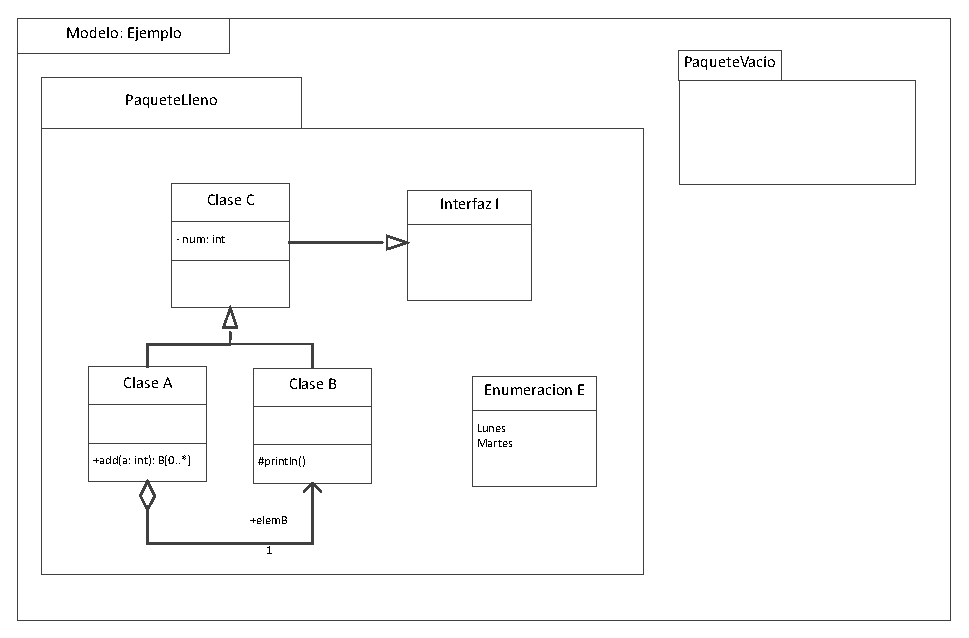
\includegraphics[width=.75\linewidth]{domainEngineering/images/Transformaciones.eps} \\
  \caption{Ejemplo de Modelo UML simplificado}
  \label{dom:fig:ejemplo}
\end{figure}


Como hemos comentado, el primer paso para desarrollar una transformaci�n de modelo a c�digo es: (1) identificar los distintos casos o tipos de entrada con los que nos podemos encontrar; y (2) hallar un equivalente en el lenguaje destino (C\# en nuestro caso). A continuaci�n, mostramos los casos identificados (c�mo t�tulo de cada subsecci�n), y por cada caso, comentamos las equivalencias propuestas. Ciertas de estas reglas son espec�ficas para l�neas de productos software, mientras que otras, como la transformaci�n de las asociaciones, son aplicables a cualquier transformaci�n de UML 2.0 a C#.
Cada regla de transformaci�n la ilustramos utilizando el ejemplo de la Figura~\ref{back:fig:smartHome}.

\subsection{Modelo}

Un modelo UML, es decir, el elemento ra�z que contiene al resto de los elementos de un modelo UML, se transforma en el \emph{namespace} para el proyecto C\#. Los \emph{namespaces} permiten agrupar entidades tales como paquetes, clases, objetos y funciones bajo el mismo nombre. De esta forma, se pueden tener varios \emph{namespaces} en el mismo proyecto que son independientes entre s�.

Recordar que para que varias clases parciales puedan ser combinadas, �stas deben pertenecer a un mismo \emph{namespace}. Por tanto, se utiliza como nombre de dicho \emph{namespace}, el nombre del modelo UML 2.0 que sirve de entrada a los generadores de c�digo.

Adem�s, al transformar el modelo UML 2.0, se crea un proyecto Visual Studio 2010, inicialmente vac�o, con el mismo nombre que el modelo UML 2.0.

Para el caso de la Figura~\ref{back:fig:smartHome}, el nombre del modelo, el cual no aparece en el diagrama, es \emph{SmartHome}. Por tanto, se crear�a un proyecto Visual Studio 2010, con \emph{SmartHome} como nombre. Dentro de dicho proyecto, se crear�a un \emph{namespace} denominado \emph{SmartHome}.

\subsection{Paquete}

Cada paquete UML 2.0 representa en nuestro caso una familia de clases, la cual encapsula una caracter�stica. Por tanto, por cada paquete UML 2.0, se crea una nueva carpeta o directorio, con el mismo nombre que el paquete, en el proyecto Visual Studio 2010 creado al transformar el modelo que contiene dicho paquete. En dicho directorio se colocar�n todos los ficheros resultantes de transformar el contenido de dicho paquete.

Por ejemplo, para el caso de la Figura~\ref{back:fig:smartHome}, durante la transformaci�n del paquete \imp{WindowMng}, se crear�a una nueva carpeta dentro del proyecto Visual Studio 2010 generado, denominada \imp{WindowMng}. Lo mismo se aplicar�a al resto de los paquetes.

\subsection{Tipos primitivos}
\label{subsec:domain:primitiveType}

Por cada tipo primitivo de UML 2.0, se establece una correspondencia con los tipos primitivos de C\#. Por ejemplo, un \emph{String} de UML 2.0 se transforma en \emph{String} de C\#. Un \emph{boolean} de UML 2.0 se transforma en un \emph{bool} de C\#. Esta correspondencia es bastante directa y no presenta problemas m�s de all� de tener que renombrar algunos tipos.

\subsection{Clases Enumeradas}

Cada clase enumerada UML 2.0, se transforma en un enumerado de C\#, con el mismo nombre que el enumerado UML 2.0. A continuaci�n, se procesan los literales de la clase enumerado UML 2.0, a�adiendo un literal con el mismo nombre al enumerado creado en C#.

Por ejemplo, la clase enumerada \imp{TempUnits} de la caracter�stica \imp{HeaterMng} se transformar�a en un enumerado de C\#, con nombre \imp{TempUnits}, perteneciente al \emph{namespace} \imp{HeaterMng}, y con \imp{CELSIUS} y \imp{FARENHEIT} como literales. El Listado~\ref{dom:code:enum} muestra el c�digo resultante de esta transformaci�n.

\begin{lstlisting} [basicstyle=\ttfamily\scriptsize,language=CSharp, captionpos=b,
                    caption=C�digo generado para la clase enumerada \imp{TempUnits},
                    label=dom:code:enum]
01 namespace SmartHome{
02    enum TempUnits {
03        CELSIUS,
04        FARENHEIT
05    };
06 }
\end{lstlisting}

\subsection{Clase}
\label{subsec:domain:class}
Por cada clase UML 2.0 encontrada dentro de un paquete, se genera una clase parcial sita en el directorio correspondiente al paquete al cual pertenece. El nombre de la clase parcial es el mismo que el de la clase UML 2.0.

Por ejemplo, para la clase \emph{WindowCtrl}, del paquete \emph{WindowMng}, se crear�a una clase parcial p�blica, denominada \emph{WindowCtrl}, y sita en la carpeta del proyecto \emph{WindowMng}.

A continuaci�n, se procesan los contenidos de dicha clase, tal como se describe a continuaci�n.

\subsection{Atributo}
\label{subsec:domain:atrib}
Cada atributo de una clase en UML 2.0 se transforma en una propiedad de C\#, perteneciente a clase parcial correspondiente a la clase que posee el atributo en el modelo UML 2.0. Dicha propiedad tendr� siempre visibilidad \emph{protegida} (\emph{protected}), salvo que estuviese declarada como \emph{privada} (\emph{private}) en el modelo UML 2.0, en cuyo caso se mantendr� la visibilidad privada.

Si el atributo era p�blico en el modelo UML, se le generar�n m�todos de acceso (\emph{getter} y \emph{setter}) a dicha propiedad. Si el atributo fuese de solo lectura o derivado, no se le generar�a m�todo de escritura (\emph{setter}).

Si el atributo fuese est�tico (\emph{static}), se generar� como est�tico en el c�digo C\#, y no se le generar�n m�todos de acceso.

Si el tipo del atributo es un tipo primitivo y el atributo no es multivaluado, es decir, la cota superior de su multiplicidad es igual a 1, se utiliza como tipo su correspondiente en C\#, de acuerdo las correspondencias comentadas en la Secci�n~\ref{subsec:domain:primitiveType}. Si el tipo fuese una clase u otro tipo no primitivo, el tipo ser� el nombre resultante de transformar dicho elemento no primitivo.

Por ejemplo, el atributo \imp{id} de la clase \imp{Actuator}, dentro de la caracter�stica \imp{BaseSystem}, se transformar�a en una propiedad llamada \imp{id}, de la clase \imp{Actuator}, sita en la carpeta \imp{BaseSystem}, y perteneciente al \emph{namespace} \imp{SmartHome}. Como tipo para dicha propiedad, se utilizar�a \imp{Int}.

Para el caso del atributo \imp{units} de la clase \imp{Actuator}, dentro de la caracter�stica \imp{HeaterMng}, se utilizar�a como tipo \imp{TempUnits}, ya que ser�a �ste el nombre del enumerado resultante de transformar la clase enumerada que sirve como tipo de este atributo.

Si el atributo fuese un atributo un atributo multivaluado, es decir, la cota superior de su multiplicidad es superior a 1, el tipo de la propiedad generada ser� una colecci�n que use como tipo base el tipo del atributo. Dependiendo de ciertas propiedades del atributo \imp{isOrdered} e \imp{isUnique}, se deber� utilizar un tipo de colecci�n u otro:

%\todo{Explicar el tipo de colecci�n elegida en cada caso y por qu�}
\begin{itemize}
  \item Si el atributo tiene la propiedad \imp{isOrdered=false} e \imp{isUnique=false} estamos ante una colecci�n que admite elementos repetidos y no precisa estar ordenada, por tanto una \imp{ICollection}.
  \item Si el atributo tiene la propiedad \imp{isOrdered=false} e \imp{isUnique=true} se trata de un conjunto \imp{ISet} ya que la colecci�n es de elementos �nicos y no es necesario que est� ordenada.
  \item Si el atributo tiene la propiedad \imp{isOrdered=true} e \imp{isUnique=false} se corresponde con una propiedad de tipo lista \imp{IList} porque son elementos en los que el orden es relevante y admite repeticiones.
  \item En �ltimo lugar, si el atributo tiene la propiedad \imp{isOrdered=true} e \imp{isUnique=true} estamos ante un caso raro y no utilizado del que no se conocen equivalencias en lenguaje C\# por lo que realiza una transformaci�n a \imp{IList}, haciendo saber al usuario final durante el proceso que se ha realizado dicha transformaci�n, en el caso de que fuera necesaria.
\end{itemize}
 
\subsection{Extremos de asociaci�n}
Por cada asociaci�n entre clases en UML 2.0 se transforma en una asociaci�n C\#. Estas asociaciones pueden ser de dos tipos:
\begin{itemize}
  \item Unidireccional. Por ejemplo, la asociaci�n \imp{indoorThem} de la caracter�stica \imp{SmartEnergyMng} indica que la clase \imp{Gateway} de dicha caracter�stica dispone de una propiedad de tipo \imp{ThermometerCtrl} de car�cter monovaluado puesto que presenta multiplicidad 1. Por otro lado, en la asociaci�n \imp{actuators} de la caracter�stica \imp{InitialModel} se aprecia que dicha propiedad es de car�cter multivaluado en tal caso se proceder�a a analizar el tipo de colecci�n de la que se trata tal como se describi� en la Secci�n \ref\label{subsec:domain:atrib}.
  \item Bidireccional. Aquellos casos en los que la asociaci�n tiene lugar en ambos sentidos y por tanto las dos clases involucradas poseen atributos de la otra y viceversa. Dependiendo del tipo de bidireccionalidad (one to one, one to many o many to many) se a�aden los atributos y m�todos adicionales necesarios para implementar el correcto funcionamiento de dicha asociaci�n, se profundizar� sobre este tipo de asociaciones en la Secci�n \ref{domain:sec:ejcomplejo}.
\end{itemize} 

\subsection{Generalizaci�n}
Por cada generalizaci�n en UML 2.0 se transforma en una generalizaci�n C\#. Estas generalizaciones pueden ser de dos tipos:
   \begin{itemize}
  \item Simple. Por ejemplo, la generalizaci�n en la caracter�stica \imp{WindowMng} de la clase \imp{WindowCtrl} respecto a la clase \imp{Actuator} quedar�a reflejado en un cambio de la declaraci�n de dicha clase parcial de forma que pasar�a de estar definida como: \imp{partial class WindowCtrl} a estar definida as�: \imp{partial class WindowCtrl : Actuator}
  \item M�ltiple. Cuando una clase de una caracter�stica posee varias generalizaciones se deben crear interfaces equivalentes a dichas clases a generalizar ya que en C\# no se permite la herencia m�ltiple de varias clases pero s� de varias interfaces. Se profundizar� sobre este tipo de generalizaciones en la Secci�n \ref{domain:sec:ejcomplejo}.
\end{itemize}
    
\subsection{Operaci�n}
Cada operaci�n de una clase en UML 2.0 se transforma en un m�todo de C\#, perteneciente a clase parcial correspondiente a la clase que posee la operaci�n en el modelo UML 2.0. Dicho m�todo tendr� siempre la visibilidad privada (\emph{private}) y ser� renombrado acorde al Patr�n Slicer. Adem�s para evitar posibles conflictos, todos los m�todos ser�n virtuales. Los m�todos con visibilidad \emph{protected} no se modificar�n a visibilidad privada para respetar la visibilidad requerida inicialmente por el usuario.

Por ejemplo, el m�todo \imp{openWindow} de la clase \imp{Gateway} perteneciente a la caracter�stica \imp{SmartEnergyMng} ser� renombrado como \imp{SmartEnergyMng\_openWindow} en la correspondiente clase parcial \imp{Gateway} dentro de la carpeta del proyecto \imp{SmartEnergyMng}.

Las operaciones cuentan con par�metros que se describen a continuaci�n.

\subsection{Par�metro}
Las operaciones presentan dos tipos de par�metros: de entrada o de retorno. Para ambos de procede de forma an�loga al tratamiento de los atributos descritos en la Secci�n \ref{subsec:domain:atrib}. Por ejemplo, la operaci�n mencionada en la secci�n anterior, \imp{openWindow}, cuenta con un par�metro de entrada \imp{id} de tipo primitivo en este caso \imp{Integer}, es una operaci�n de tipo \imp{void} ya que no dispone de un par�metro de retorno asociado. 

\subsection{Constructor}
Cada clase parcial generada a partir de cada clase UML 2.0 encontrada dentro de un paquete en el modelo, implementa un m�todo privado que se corresponde con la porci�n de constructor para dicha clase en dicha caracter�stica.

Por ejemplo, para la clase parcial \imp{Gateway} de la caracter�stica \imp{HeaterMng}, se genera un m�todo denominado \imp{HeaterMng\_initGateway}. De manera an�loga, para la clase parcial \imp{Gateway} de la caracter�stica \imp{WindowMng}, se genera un m�todo denominado \imp{WindowMng\_initGateway} y as� sucesivamente.

\subsection{Interfaz}
La generaci�n de interfaces se realiza de forma an�loga a la generaci�n de clases tal como se ha explicado en la Secci�n \ref{subsec:domain:class}.



%%===================================================================%%


A continuaci�n se procede al an�lisis m�s detallado de cada uno de los elementos de dicha tabla, para ello nos apoyaremos en la Figura~\ref{dom:fig:ejemplo}.

\begin{lstlisting} [basicstyle=\ttfamily\scriptsize,language=CSharp, captionpos=b,
                    caption=C�digo generado para las clases y la interfaz del modelo de la figura \ref{dom:fig:ejemplo},
                    label=dom:code:ejemplo]
File PaqueteLleno/B.cs
--------------------------------------------------------
01 namespace Ejemplo{
02     partial class B: C{
03          ...
04          private virtual void B_initB ( ) {}
05          protected virtual PaqueteLleno_println ( ) {}
06     }
07 }

File PaqueteLleno/A.cs
--------------------------------------------------------
08 namespace Ejemplo{
09     partial class A: C{
10          private B elemB;
11          public B elemB {
12              get { return this.elemB; }
13              set { this.elemB= value; }
14          }
15          ...
16          private virtual void A_initA ( ) {}
17          private virtual ISet<B> PaqueteLleno_add (int a) { }
18     }
19 }

File PaqueteLleno/C.cs
--------------------------------------------------------
20 namespace Ejemplo{
21      partial class C: I{
22          private int num;
23          public int num {
24              get { return this.num; }
25              set { this.num= value; }
26          }
27          ...
28          private virtual void C_initC ( ) {}
29      }
30 }

File PaqueteLleno/I.cs
--------------------------------------------------------
31 namespace Ejemplo{
32     partial interface I{			
33          public virtual override bool Equals (Object o);
34          public virtual override int CompareTo (Object o);
35          public virtual override int GetHashCode ( );
36          public virtual override Type GetType ( );
37          public virtual override string ToString( );
38          private virtual void I_initI ( ) {}
39     }
40 }

File PaqueteLleno/E.cs
--------------------------------------------------------
41 namespace Ejemplo{	
42     enum E {	
43        Lunes,
44        Martes,
45     };
46 }
\end{lstlisting}

El modelo de la figura \ref{dom:fig:ejemplo} es \imp{Ejemplo} y por tanto cada clase del proyecto deber�a comenzar definiendo el namespace del modelo en cuesti�n mediante la l�nea de c�digo C\# tal como se aprecia en las l�neas 1, 8, 20, 31 y 41 del listing \ref{dom:code:ejemplo}.

En la figura \ref{dom:fig:ejemplo} hay dos paquetes \imp{PaqueteLleno} y \imp{PaqueteVac�o}, por tanto, en el directorio destino donde se generan los ficheros del modelo deber�n aparecer dos carpetas con dichos nombres. La carpeta \imp{PaqueteLleno} contendr� en su interior cuatro ficheros denominados A.cs, B.cs, C.cs, I.cs y E.cs, uno por cada clase, clase enumerada (listing \ref{dom:code:ejemplo} 41-46) o interfaz que se encuentra en su interior, mientras que la carpeta \imp{PaqueteVac�o} no contendr� ning�n archivo en su interior.

Tal como se aprecia en la figura \ref{dom:fig:ejemplo}, la clase \imp{A} del paquete \imp{PaqueteLleno}, tiene un atributo llamado \imp{num} por lo que se genera una propiedad con sus respectivos m�todos getter y setter tal como se muestra en el listing \ref{dom:code:ejemplo} en las l�neas 22-26.

La figura \ref{dom:fig:ejemplo} presenta la clase \imp A con una operaci�n \imp{add} que tiene un par�metro \imp{a: int} y retorna una colecci�n de elementos de tipo \imp{B} (listing \ref{dom:code:ejemplo} l�nea 17). De la misma forma, la clase \imp{B} tiene una operaci�n \imp{println} de car�cter \emph{protected} y por tanto su visibilidad no se transforma en \emph{private} (listing \ref{dom:code:ejemplo} l�nea 5). Con este ejemplo quedan ilustrados los puntos de operaci�n y par�metro descritos en la tabla \ref{dom:fig:tranf}.

Para la generaci�n de clases e interfaces de la figura \ref{dom:fig:ejemplo}, el resultado ser�a el mostrado en las l�neas 2, 9, 21 y 32 del listing \ref{dom:code:ejemplo}. Se aprecia tambi�n las herencias correspondientes.

Aunque no est� reflejado en el modelo UML a�adimos a cada clase, o interfaz, del modelo a�adimos un constructor (listing \ref{dom:code:ejemplo} l�neas 4, 16, 28 y 38) y unos m�todos de utilidad (listing \ref{dom:code:ejemplo} l�neas 33-37).

Por �ltimo, la asociaci�n simple de las clases \imp{A} y \imp{B} se traduce con las l�neas de c�digo descritas en las l�neas 10-14 del listing \ref{dom:code:ejemplo}.

Con esto queda explicado m�s detalladamente la transformaci�n de modelo UML a c�digo C\# descrita en la tabla \ref{dom:fig:tranf}. Se han omitido la herencia m�ltiple y las asociaciones bidireccionales por su complejidad. En la siguiente secci�n se profundizar� en la implementaci�n y creaci�n de las transformaciones de modelo UML a c�digo C\#.


\section{Generadores de C�digo C\#}
\label{domain:sec:gen}
%%==================================================================%%
%% Author : Abascal Fern�ndez, Patricia                             %%
%% Author : S�nchez Barreiro, Pablo                                 %%
%% Version: 2.9, 25/04/2013                                         %%
%%                                                                  %%
%% Memoria del Proyecto Fin de Carrera                              %%
%% Domain Engineering/Generadores de C�digo C#                      %%
%%==================================================================%%

Para implementar los generadores de c�digo, se procedi� en encapsular cada una de las reglas descritas en la secci�n anterior en un \emph{template} de EGL. Adem�s, se crearon una serie de funciones auxiliares en EOL. Por ejemplo, se cre� una funci�n auxiliar para determinar el tipo de colecci�n que debe ser utilizada para transformar un atributo multivaluado, es decir, con cota superior de su multiplicidad mayor que uno.

Uno de los mayores problemas que normalmente plantean los generadores de c�digo es que la generaci�n de c�digo es secuencial, no permitiendo la vuelta a atr�s. Por ejemplo, si generamos una clase y m�s tarde descubrimos que dicha clase debe ser modificada porque act�a como clase padre en una herencia m�ltiple, ya no podremos volver a abrir dicha clase para a�adirle la relaci�n de herencia con la interfaz que ha de crearse.

Por tanto, antes de generar una clase, debemos asegurarnos de que no va a necesitar ser modificada posteriormente. Ello implica que hay que tener especial cuidado a la hora de dise�ar el orden en el cual se ejecutan las plantillas, o \emph{templates} de generaci�n de c�digo. La Figura~\ref{dom:fig:templates} muestra el orden de ejecuci�n de las plantillas creadas en nuestro caso. Explicamos parte de dicha figura, aunque no la describiremos entera, por razones de espacio.

\begin{figure}[!tb]
  \center
  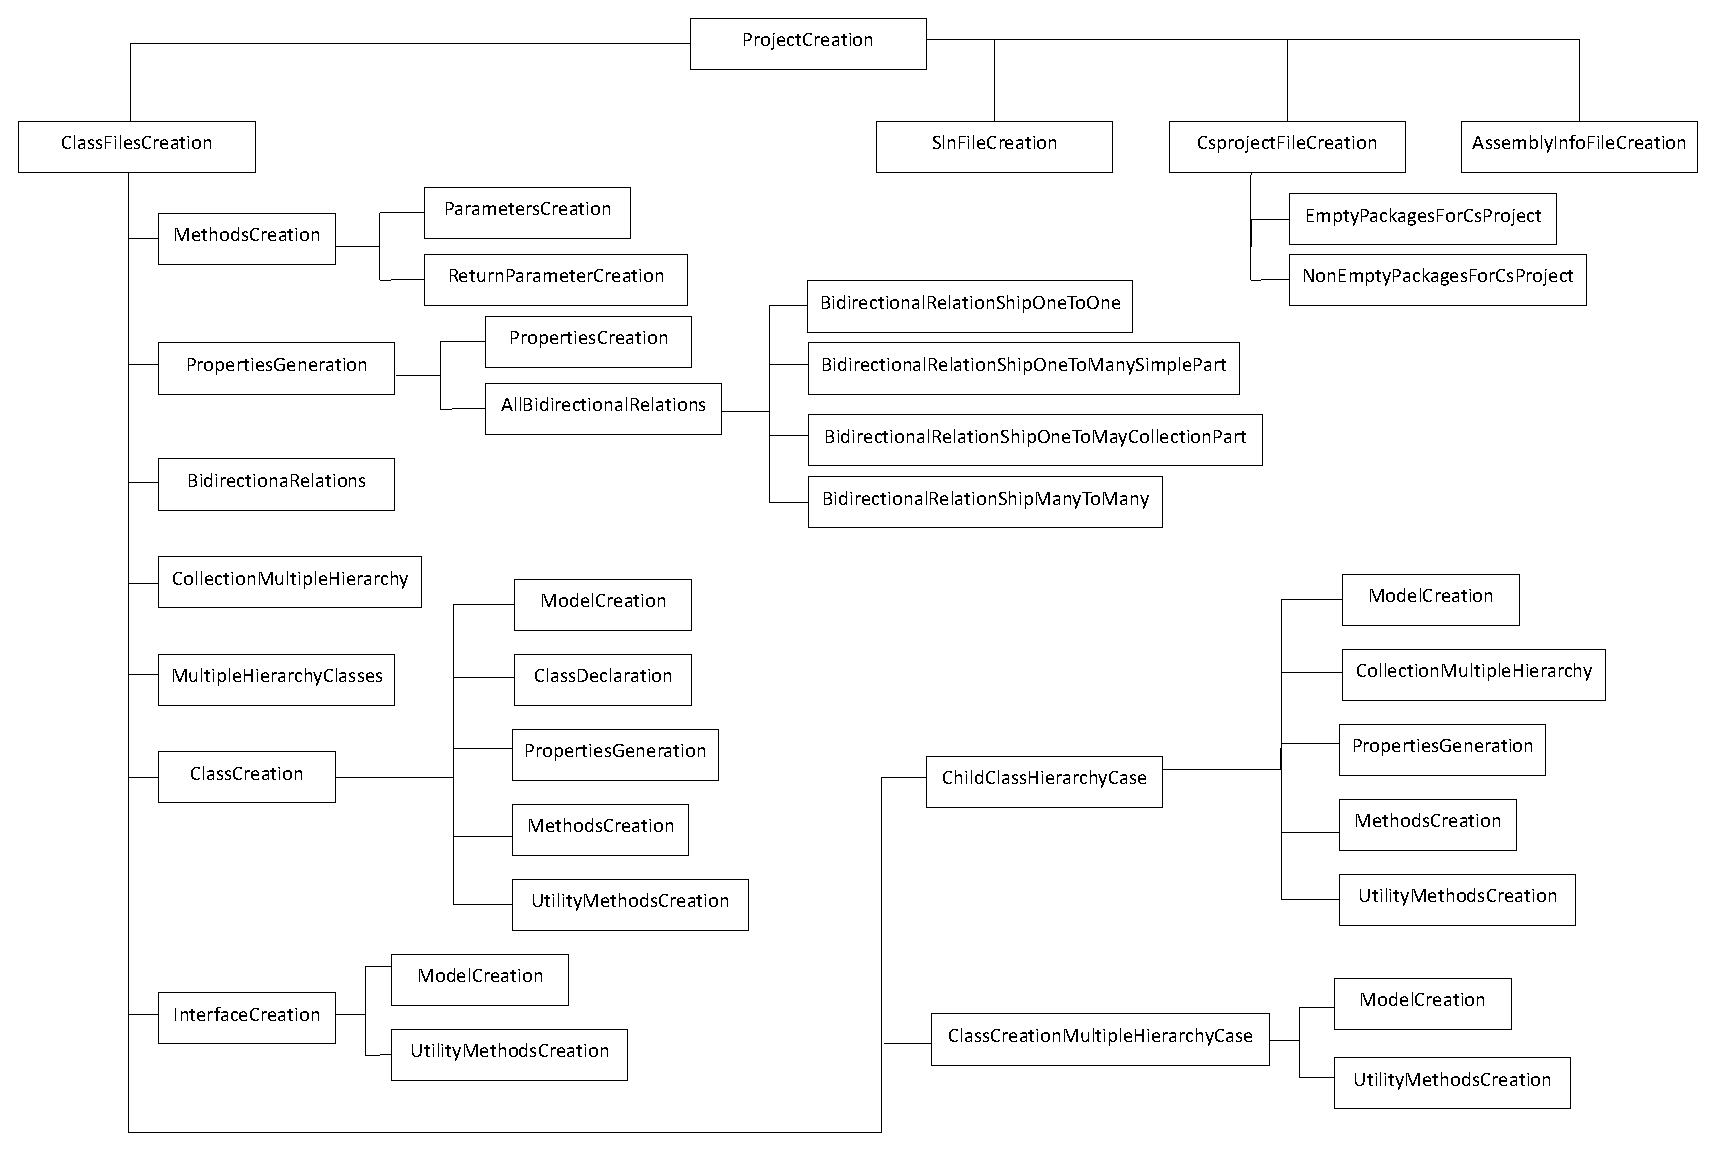
\includegraphics[width=\linewidth]{domainEngineering/images/Templates.eps} \\
  \caption{Orden de ejecuci�n de las plantillas de generaci�n de c�digo}
  \label{dom:fig:templates}
\end{figure}

El punto de partida es el generador de c�digo llamado \imp{ProjectCreation}, encargado de procesar el elemento \emph{modelo}, que constituye la ra�z del proyecto, as� como los \emph{paquetes} que contiene dicho modelo, adem�s de crear el proyecto \emph{Visual Studio 2010} que constituye la salida del generador.  Dicho \emph{template} tiene , por tanto, dos tareas claramente diferenciadas: (1) por una parte, debe generar el c�digo correspondiente a la arquitectura de referencia, lo que se hace a trav�s de la plantilla \imp{ClassFilesCreation}; y (2) por otra parte, debe generar todos los ficheros auxiliares y la estructura que constituyen un proyecto \emph{Visual Studio 2010}, como el fichero de construcci�n (fichero \emph{.csproj}) que indica que clases parciales deben compilarse cuando se construye el proyecto (ver Figura~\ref{back:code:partialClasses}). Para generar estos ficheros auxiliares, se utilizan las plantillas \imp{SlnFileCreation},  \imp{CsprojectFileCreation} y \imp{AssemblyInfoFileCreation}.

La plantilla \imp{ProcessPackageContents} procesa por cada paquete, su contenido. Dependiendo del tipo de cada elemento, se realiza una acci�n diferente, tal como se describe a continuaci�n.

Si se trata de una clase enumerada, se invoca el template \imp{EnumerationClassCreation}, con dicho elemento como argumento.

Se procesan todas las clases con herencia m�ltiple, para aplicar el \emph{mixin pattern}. Para ello se ejecutan las plantillas \imp{ParentImplMultipleInheritanceCase}, que se encarga de procesar las clases padre involucradas en herencias m�ltiples; y \imp{ParentInterfaceMultipleInheritanceCase}, que se encarga de crear las interfaces para estas clases padre. Ambas plantillas hacen uso de las plantillas \imp{MethodsCreation} y \imp{UtilityMethodsCreation}, encargadas de procesar los m�todos de dichas clases e interfaces y de crear los m�todos de infraestructura que fuesen necesarios, tal como \imp{Equals} o \imp{CompareTo}.

A continuaci�n, se ejecuta la plantilla \imp{ChildClassMultipleInheritance}, encargada de procesar una clase hija involucrada en herencia m�ltiple. Para ello se procesan el esqueleto de la clase \imp{ClassDeclaration}, sus atributos (\imp{PropertiesGeneration}), sus m�todos \imp{MethodsCreation} y sus m�todos de infraestructura \imp{UtilityMethodsCreation}.

Seguidamente, se procesan las clases no afectadas, como hijas o como padres, por herencia m�ltiple. Estas clases se procesan a trav�s de la plantilla \imp{ClassCreation}, que funciona igual que la plantilla \imp{ChildClassMultipleInheritance}, a excepci�n de que no se genera el c�digo de los delegados para los \emph{mixins}.

Cada plantilla invocada hace uso a su vez de otras subplantillas, que por razones de claridad y espacio no detallamos. Por ejemplo, la plantilla \imp{PropertiesGeneration} encargada de procesar atributos y extremos de asociaci�n, hace uso de diversas plantillas para procesar los extremos pertenecientes a asociaciones doblemente navegables, tal como se indica en la Figura~\ref{}.

Por �ltimo, comentar que todas las plantillas utilizan diversas funciones auxiliares especificadas en EOL. Por ejemplo, existen funciones para determinar si una clase est� involucrada en una herencia m�ltiple o para devolver todas las clases padre de una clase dada. Adem�s, junto con las funciones auxiliares de EOL, se han creado una serie de funciones auxiliares en Java, invocables desde EOL, y EGL, lo que se conoce en argot Epsilon como una \emph{Java Tool}, para poder manipular el sistema de ficheros. Esto era necesario, por ejemplo, para poder crear la estructura de carpetas del proyecto Visual Studio 2010.

Adem�s, se crearon algunas \emph{Java Tool} para poder mostrar cuadros de di�logo que permitiesen inteactuar con el usuario durante el proceso de generaci�n de c�digo, ya fuese para mostrarle o requerirle informaci�n.

\begin{figure}[!tb]
  \centering
  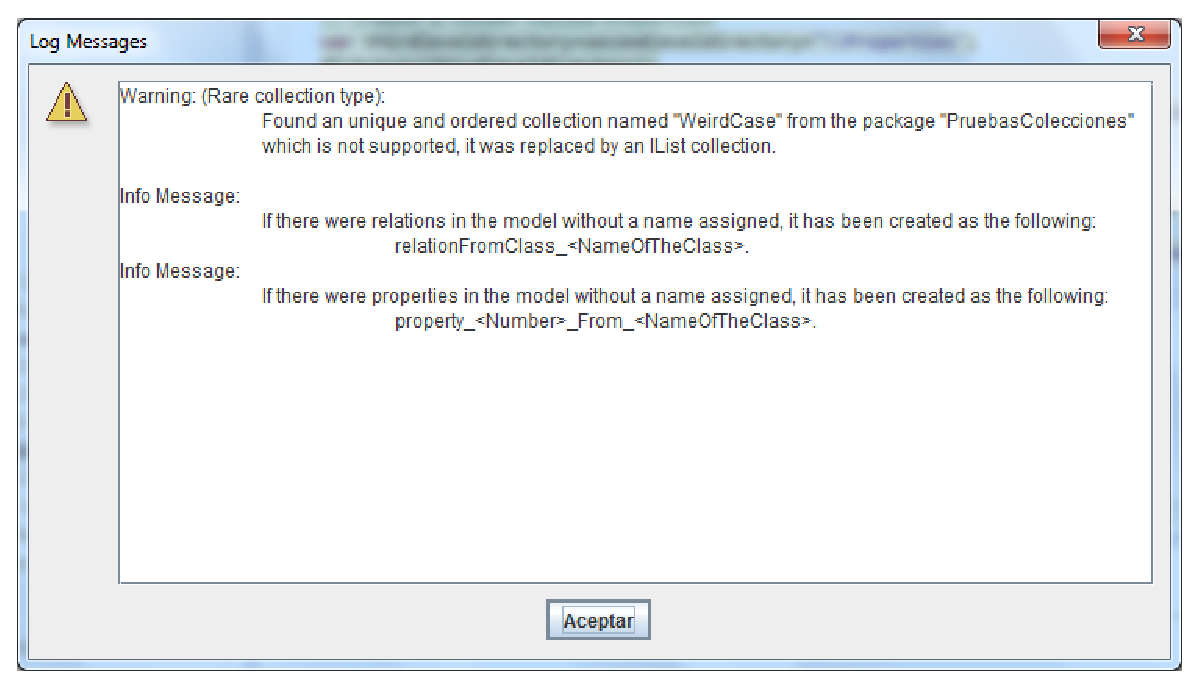
\includegraphics[width=.75\linewidth]{domainEngineering/images/FinalWindow.eps} \\
  \caption{Log mostrado al finalizar el proceso}
  \label{dom:fig:final}
\end{figure}


Las Figuras~\ref{} y~\ref{dom:fig:final} muestra dos ejemplos de estos di�logos. El primero de ellos aparecer�a al utilizar como entrada para el generador de c�digo un archivo UML que tuviese varios modelos. En este caso, el proceso de generaci�n de c�digo preguntar�a al usuario cu�l es el modelo a procesar, ya dentro de un fichero UML pueden coexistir modelos de diversa �ndole.

El segundo di�logo (Figura~\ref{dom:fig:final}) muestra, al final del proceso de generaci�n de c�digo, las incidencias que hayan podido producirse durante dicho proceso. 

La siguiente secci�n muestra, para el lector interesado, una plantilla de las descritas en esta secci�n a nivel de c�digo. 

\section{Ejemplo de Generaci�n de C�digo C\#: Caso Sencillo}
\label{domain:sec:ejsencillo}
%%==========================================================================%%
%% Author : Abascal Fern�ndez, Patricia                                     %%
%% Author : S�nchez Barreiro, Pablo                                         %%
%% Version: 1.1, 21/04/2013                                                 %%
%%                                                                          %%
%% Memoria del Proyecto Fin de Carrera                                      %%
%% Domain Engineering/Ejemplo de Generaci�n de C�digo C#: Caso Sencillo     %%
%%==========================================================================%%
\begin{figure}[tb!]
\begin{center}
\begin{footnotesize}
\begin{verbatim}
01 [%import "ReturnParameterCreation.egl";
02 import "ParametersCreation.egl";
03 import "../Operations.eol";
04 operation Element classMethods(currentPackage: String, path: String): String {   		
05  ...
06  opers=private()+void()+currentPackage+"_init"
          +self.firstToUpperCase()+" ( ) {}\n\t\t";
07  ...
08  for (oper in self.getOperations()){
09      for (par in oper.ownedParameter){
10          ...	
11          if (oper.type==null){
12              isReturn=false;
13          }else{
14              if (par.direction.toString().equals("return")){
15                  if (not par.type.name.isDefined()){
16                      isReturn=false;
17                  }else{
18                      isReturn=true;
19                  }//if-par-type
20              }//if-par-direction
21          }//if-oper-type
22      }//for-parameters
23      if (isReturn){
24          operations_return.add(oper);
25      }else{
26          operations_void.add(oper);
27      }		
28  }//for-operations	
29  for (oper in operations_void) {
30      if (oper.name==""){
31          methodname="method_"+iter;
32      }else{
33          methodname=oper.name;
34		}
35      opers=opers+oper.visibility()+oper.abstract()+oper.esStatic()+virtual()
              +void()+currentPackage+"_"+methodname
              +" ("+oper.parameters(currentPackage, path)+") {}\n\t\t";
36      // Increase the iterator
37      iter=iter+1;
38  }
39  for (oper in operations_return) {
40      if (oper.name==""){
41          methodname="method_"+iter;
42      }else{
43          methodname=oper.name;
44      }
45      opers=opers+oper.visibility()+oper.abstract()+oper.esStatic()+virtual()
             +oper.returnParameter(currentPackage, path)+" "+currentPackage+"_"+methodname
             +" ("+oper.parameters(currentPackage, path)+") {}\n\t\t";
46      // Increase the iterator
47      iter=iter+1;
48  }
49  return opers;
50 }%]
\end{verbatim}
\end{footnotesize}
\end{center}
\caption{Implementaci�n del generador de c�digo \imp{MethodsCreation}}
\label{dom:code:method}
\end{figure}

Para introducir al lector en la implementaci�n de los generadores de c�digo, vamos a analizar en detalle uno de los generadores de c�digo m�s sencillos: \imp{MethodsCreation}, el fichero fuente aparece en la figura \ref{dom:code:method}. Vamos a proceder al an�lisis detallado del mismo:
\begin{itemize}
  \item L�neas 1-3, generadores de c�digo que utiliza y fichero \imp{Operations.eol} que contiene las funciones b�sicas comunes a los generadores de c�digo.
  \item L�nea 4, descripci�n de la funci�n que retornar� el texto generado.
  \item L�nea 6, texto correspondiente al constructor de la clase de la forma $<$nombre del paquete$>$\_init$<$nombre de la clase$>$.
  \item L�neas 8-28, tratamos una a una todas las operaciones descritas en elemento actual (clase o interfaz).
  \item L�neas 9-22, en cada operaci�n recorremos todos y cada uno de los par�metros.
  \item L�neas 11-13, si la operaci�n no tiene definido un tipo, es decir, si el usuario ha obviado especificar si la funci�n devuelve una colecci�n, un entero, un elemento de una clase, etc, por defecto se trata como una operaci�n void (operaci�n que no retorna ning�n valor).
  \item L�nea 15, si la operaci�n tiene un tipo de retorno definido, comprobamos si dicho par�metro es de retorno.
  \item L�nea 16, si el par�metro es de retorno pero no est� definido vuelve a ser tratada como una operaci�n void.
  \item L�nea 18, si el par�metro es de retorno y tiene un tipo definido se trata de una operaci�n que s� retorna un valor.
  \item L�nea 24, si la operaci�n que est� siendo analizada retorna un valor, se a�ade a la lista de operaciones que devuelven un valor.
  \item L�nea 26, si la operaci�n que est� siendo analizada no retorna un valor, se a�ade a la lista de operaciones que no devuelven un valor.
  \item L�nea 29-38, a�adir al string resultado la informaci�n correspondiente a los m�todos de la clase actual que no retornan ning�n valor (m�todos void).
  \item L�nea 31, si el m�todo no tiene un nombre definido, se otorga un nombre por defecto.
  \item L�nea 35, se realizan llamadas a los generadores de c�digo para obtener los par�metros de la funci�n.
  \item L�nea 39-48, de manera an�loga a las operaciones que no retornan ning�n valor, se procede a a�adir al string resultado los m�todos de la clase que s� retornan un valor.
  \item L�nea 49, se retorna el string con todos los m�todos de la clase o interfaz actual.
\end{itemize}

Un vez explicado un ejemplo sencillos, las siguiente secci�n {domain:sec:ejcomplejo} explica ejemplos m�s complejos que quedan a la curiosidad del lector.



\section{Ejemplo de Generaci�n de C�digo C\#: Caso Complejo}
\label{domain:sec:ejcomplejo}
%%==========================================================================%%
%% Author : Abascal Fern�ndez, Patricia                                     %%
%% Author : S�nchez Barreiro, Pablo                                         %%
%% Version: 1.2, 23/04/2013                                                 %%
%%                                                                          %%
%% Memoria del Proyecto Fin de Carrera                                      %%
%% Domain Engineering/Ejemplo de Generaci�n de C�digo C#: Caso Complejo     %%
%%==========================================================================%%
Antes de comenzar a exponer los ejemplos m�s complejo, vamos a introducir aquellos conceptos que pasamos por algo en la secci�n \ref{domain:sec:transf} dada su complejidad: las relaciones bidireccionales y la herencia m�ltiple.

 \paragraph{Relaciones Bidireccionales} \ \\
 \begin{figure}[!tb]
  \centering
  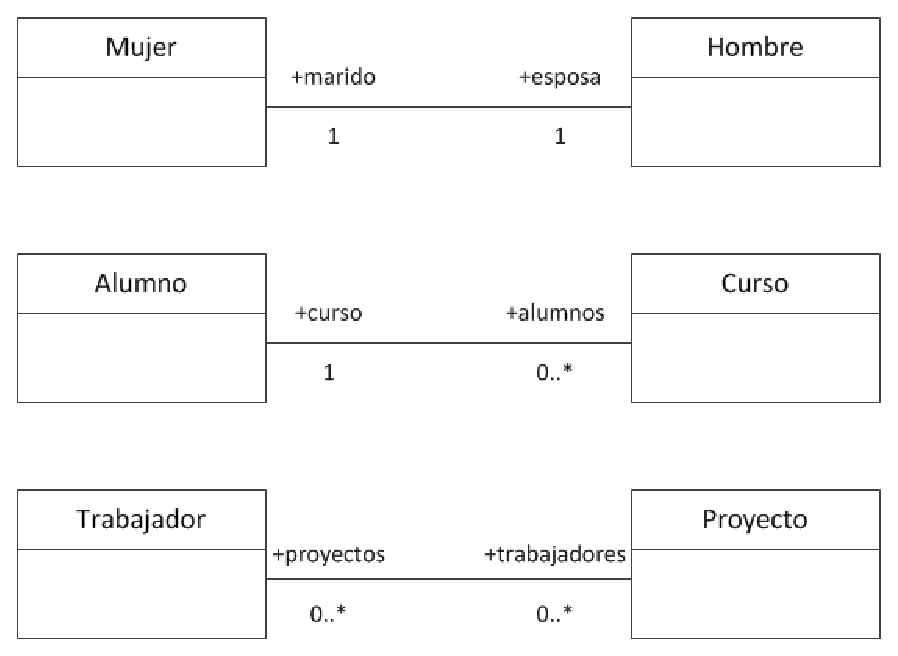
\includegraphics[width=.75\linewidth]{domainEngineering/images/bidireccionales.eps} \\
  \caption{Tipos de relaciones bidireccionales}
  \label{dom:fig:bid}
\end{figure}

Las relaciones bidireccionales son aquellas en las que ambas clases relacionadas disponen de atributos de la clase opuesta. Existen tres tipos de relaciones bidireccionales:
 \begin{itemize}
   \item \emph{Bidireccionalidad one to one}, en las que cada clase recibe un elemento de la clase opuesta (figura \ref{dom:fig:bid}, Mujer-Marido).
   \item \emph{Bidireccionalidad one to many}, en la que una de las clases recibe un elemento de la clase destino y la otra recibe una colecci�n de elementos de la clase opuesta (figura \ref{dom:fig:bid}, Alumno-Curso).
   \item \emph{Bidireccionalidad many to many}, en la que ambas clases reciben colecciones de la clase opuesta (figura \ref{dom:fig:bid}, Trabajadores-Proyectos).
 \end{itemize}

 Llegados a este punto, bas�ndonos en los ejemplos de la figura \ref{dom:fig:bid} nos surgen algunas preguntas:
 \begin{enumerate}
   \item �Si una mujer A tiene un esposo B y ese esposo B tiene una mujer que no sea A?
   \item �Si un alumno tiene asignado un curso pero ese curso no tiene a dicho alumno en su lista de alumnado?
   \item �Si un trabajador tiene asignado un proyecto pero en el listado de trabajadores dicho trabajador no aparece?
 \end{enumerate}
�Existe alguna forma de poner soluci�n a estos problemas?, la respuesta es s�, a la hora de tratar este tipo de relaciones bidireccionales en los generadores de c�digo correspondientes no basta con generar las propiedades tal como hemos estado haciendo hasta ahora sino que debemos implementar las propiedades a generar de una forma cuidadosa y exhaustiva para que no se produzcan este tipo de incoherencias, incluso recurriendo a la creaci�n de m�todos adicionales. Veamos a grandes rasgos en la tabla \ref{dom:table:bid} c�mo ser�a la implementaci�n de la relaci�n bidireccional one to one:
\begin{table}%
\begin{tabularx}{15cm}{|l|X|X|}
 \hline
{}&{\textbf{Mujer soltera}}&{\textbf{Mujer casada}} \\ \hline
{\textbf{Hombre soltero}} &
                Se casan el hombre soltero y la mujer soltera.
&  La mujer casada se divorcia. El antiguo marido de la mujer divorciada queda soltero. La mujer divorciada y el hombre soltero se casan. \\ \hline
{\textbf{Hombre casado}} & El hombre casado se divorcia. La antigua mujer del marido divorciado queda soltera. Se casan la mujer soltera y el hombre divorciado.
& El hombre casado se divorcia. La antigua mujer del marido divorciado queda soltera. La mujer casada se divorcia. El antiguo marido de la mujer divorciada queda soltero. Se casan la mujer divorciada y el hombre divorciado. \\ \hline
\end{tabularx}
\caption{Soluci�n para evitar incoherencias en el c�digo C\# en la bidireccionalidad one to one}
\label{dom:table:bid}
\end{table}%
El siguiente paso ser�a pasar dicha tabla a c�digo C\# y comprobar que funciona correctamente. Se sigue un proceso an�logo para el resto de relaciones bidireccionales.

\paragraph{Herencia m�ltiple} \ \\

\begin{figure}[!tb]
  \centering
  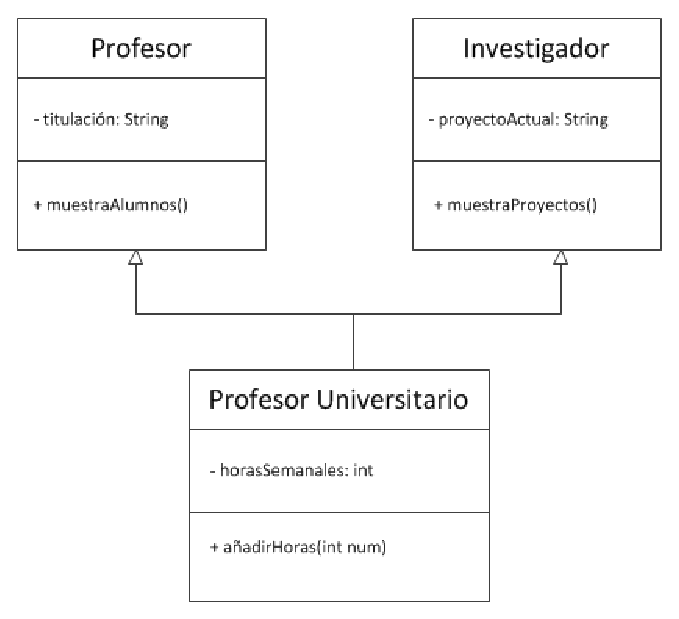
\includegraphics[width=.50\linewidth]{domainEngineering/images/herenciamultiple.eps} \\
  \caption{Tipos de relaciones bidireccionales}
  \label{dom:fig:her}
\end{figure}



\section{Pruebas con EUnit}
\label{domain:sec:pruebas}
%%==========================================================================%%
%% Author : Abascal Fern�ndez, Patricia                                     %%
%% Author : S�nchez Barreiro, Pablo                                         %%
%% Version: 1.4, 29/04/2013                                                 %%
%%                                                                          %%
%% Memoria del Proyecto Fin de Carrera                                      %%
%% Domain Engineering/Pruebas con EUnit                                     %%
%%==========================================================================%%
EUnit es un sistema de pruebas \cite{kolovos:2008} unitarias que proporciona assertions para la comparaci�n de modelos, archivos y directorios. Una \emph{assertion} es un predicado, verdadero o falso, colocado en un programa para indicar que el desarrollador cree que el predicado es siempre cierto en ese lugar. Las pruebas pueden reutilizarse con diferentes conjuntos de modelos y datos de entrada, y las diferencias entre los modelos esperados y los reales pueden ser visualizadas gr�ficamente.

Al comenzar la fase de pruebas me encontr� con el problema inicial de que EUnit no ten�a implementada la comparaci�n de fragmentos de texto en los ficheros generados que era precisamente la manera de comprobar que los generadores de c�digo funcionaban correctamente. De tal forma proced� a realizar una petici�n en el foro de la plataforma e incorporaron una nueva assertion denominada \imp{assertLineWithMatch} que permit�a comprobar si un fichero dispon�a de un determinado fragmento de texto o no (l�neas 1-4 del listing \ref{dom:code:eunit}). Tambi�n era necesario comprobar que los ficheros y directorios se creaban correctamente por lo que la assertion \imp{assertEqualDirectories} es v�lida para tal fin (l�neas 6-9 del listing \ref{dom:code:eunit}). Y por �ltimo, se debe comprobar que las plantillas lanzan las excepciones oportunas para los casos no v�lidos, mediante la combinaci�n de las instrucciones \imp{assertError} y \imp{runTarget}, se puede comprobar si el fichero deseado lanza o no una excepci�n (l�neas 11-16 del listing \ref{dom:code:eunit}). Con estas assertions se procede a realizar todos los casos de prueba descritos en la tabla \ref{dom:table:bid} con resultados satisfactorios.

\begin{lstlisting} [basicstyle=\ttfamily\scriptsize,language=CSharp, captionpos=b,
                    caption=Pruebas de los generadores de c�digo con EUnit,
                    label=dom:code:eunit]
01 @test
02 operation classWithNameAndWithoutType() {
03    assertLineWithMatch(path+"Data\\src\\BasicGraph\\Edge.cs",
                          "partial class Edge");
04 }
05 ...
06 @test
07 operation emptyPackage() {
08    assertEqualDirectories(path+"Data\\src\\PaqueteVacio",
                             path+"\\Data\\src\\PaqueteVacio");
09 }
10 ...
11 @test
12 operation thowsExceptions() {
13    ...
14    assertError(runTarget(pathTemplates+'\\ParametersCreation.egl'));
15    ...
16 }
\end{lstlisting}


\begin{table}%
\begin{tabularx}{17cm}{|l|X|l|}
 \hline
{}&{Casos v�lidos}&{Casos no v�lidos} \\ \hline
\multirow{12}{*}{Clase} & Clase con nombre. & Clase fuera de un paquete. \\
& Clase tipo abstract. & Clase sin nombre.\\
& Clase sin tipo. & Clase enumerada.\\
& Clase que hereda de una o varias clases. &\\
& Clase que hereda de una o varias interfaces. &\\
& Clase que hereda de clases e interfaces. &\\
& Clase sin propiedades. &\\
& Clase sin m�todos. &\\
& Clase sin propiedades ni m�todos. &\\
& Clase con propiedades. &\\
& Clase con m�todos. &\\
& Clase con propiedades y m�todos. &\\
\hline
\multirow{4}{*}{Paquete} & Paquete con nombre. & Paquete sin nombre. \\
& Paquete con clases e interfaces en su interior. & \\
& Paquete vac�o. & \\
& Paquete dentro de otro paquete (recursividad). & \\
\hline
\multirow{4}{*}{Clase Enumerada} & Clase enumerada con nombre. & Clase enumerada sin nombre. \\
& Clase enumerada con literales. & \\
& Clase enumerada vac�a. & \\ 
\hline
\multirow{3}{*}{Interfaz} & Interfaz con nombre. & Interfaz sin nombre. \\
& Interfaz sin m�todos. & Interfaz fuera de paquete.\\
& Interfaz con m�todos. & \\
\hline
\multirow{10}{*}{Propiedad} & Propiedad con nombre. & Propiedad sin tipo. \\
& Propiedad sin nombre (se debe poner uno por defecto). & Asociaciones sin multiplicidad.\\
& Propiedad est�tica (no lleva m�todos getter ni setter). & \\
& Propiedad protected (no lleva m�todos getter ni setter). & \\
& Propiedad no est�tica (lleva m�todos getter ni setter). & \\
& Propiedad es una colecci�n. & \\
& Propiedad es una asociaci�n simple. & \\
& Propiedad es una asociaci�n bidireccional one to one. & \\
& Propiedad es una asociaci�n bidireccional one to many. & \\
& Propiedad es una asociaci�n bidireccional many to many. & \\
\hline
\multirow{14}{*}{M�todo} & M�todo con nombre. & \\
& M�todo sin nombre (se debe poner uno por defecto). &  \\
& M�todo sin tipo (se debe poner void por defecto). &  \\
& M�todo sin tipo (se debe poner void por defecto) y sin par�metros. & \\
& M�todo sin tipo (se debe poner void por defecto) y con par�metros. &  \\
& M�todo void sin par�metros. &  \\
& M�todo void con par�metros. &  \\
& M�todo retorna tipo primitivo sin par�metros. &  \\
& M�todo retorna tipo primitivo con par�metros. &  \\
& M�todo retorna colecci�n sin par�metros. &  \\
& M�todo retorna colecci�n con par�metros. &  \\
& M�todo est�tico. &  \\
& M�todo abstracto. &  \\
& M�todo protected. &  \\
\hline
\multirow{3}{*}{Par�metros de m�todo} & Par�metro con nombre. & Par�metro sin tipo. \\
& Par�metro sin nombre (se debe poner uno por defecto). & \\
& Par�metro con tipo. & \\
\hline
\multirow{2}{*}{Herencia} & Herencia simple. &   \\
& Herencia m�ltiple (se debe implementar interfaces y clases adicionales, si fuera necesario). & \\
\hline
\end{tabularx}
\caption{Soluci�n para evitar incoherencias en el c�digo C\# en la bidireccionalidad one to one}
\label{dom:table:bid}
\end{table}%

Durante este cap�tulo se han descrito la fase de \emph{Ingenier�a del Dominio} de nuestra l�nea de productos software. Dentro de dicha fase se ha analizado c�mo se transforman los elementos del modelo a c�digo C\#, el desarrollo e implementaci�n de los generadores de c�digo junto con la explicaci�n de varios ejemplos y se ha conclu�do con la fase de pruebas.



\section{Sumario}

Durante este cap�tulo se han descrito la fase de \emph{Ingenier�a del Dominio} de nuestra l�nea de productos software. Dentro de dicha fase se ha analizado c�mo se transforman los elementos del modelo a c�digo C\#, el desarrollo e implementaci�n de los generadores de c�digo junto con la explicaci�n de varios ejemplos y se ha conclu�do con la fase de pruebas.
